\documentclass[tikz]{standalone}

\usepackage{tikz}
\usetikzlibrary{calc}
\usetikzlibrary{arrows.meta}

\begin{document}
    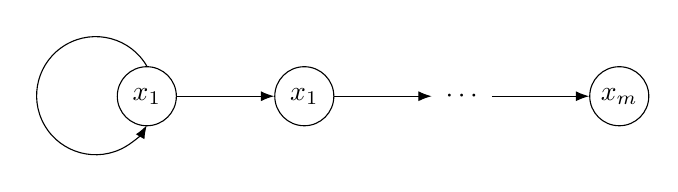
\begin{tikzpicture}[
        remember picture,
        every node/.style={draw,circle,minimum size=0.75cm,inner sep=-1pt},
        >=Latex
    ]
        \node (x1) at (0,0) {$x_1$};
        \node (x2) at ($(x1) + (0:2)$) {$x_1$};
        \node[draw=none] (xd) at ($(x2) + (0:2)$) {$\cdots$};
        \node (xm) at ($(xd) + (0:2)$) {$x_m$};
        \draw[->] (x1) -- (x2);
        \draw[->] (x2) -- (xd);
        \draw[->] (xd) -- (xm);
        \draw[->] (x1.north) arc(30:330:0.75);
    \end{tikzpicture}
\end{document}